\documentclass[12pt,a4paper]{article}
\usepackage{amsmath}
\usepackage{textcomp}
\usepackage[a4paper,margin=0.8in]{geometry} 
\usepackage{natbib}
\usepackage{longtable}
\usepackage{graphicx}
\usepackage{appendix}

\bibliographystyle{agsm}

%opening
\title{An investgation into the use of machine learning techniques as a tool in the study of the factors that affect life expectancy on a global scale}
\author{Adriaan Louw (53031377)}




\begin{document}

\maketitle

\newpage

\thispagestyle{plain}
\begin{center}
    \Large
    \textbf{Abstract}
\end{center}

\newpage

\tableofcontents

\listoffigures

\listoftables

\section{Introduction}

Human beings have always had a fascination with longevity. Myths like the fountain of youth or the Holy Grail are a testament to this fact. Today, longevity and causes of mortality are studies by profesionals like Demographers and Actuaries. Trying to determine why some people or group live long lives.    

This study investigates the use of Machine Learning techniques in studying the determinants of life expectancy for coutries. Selecting indicators that have shown to have some form of correlation with life expectancy. Their relationship with life expectancy will be investigated using various techniques from Machine Learning and contrasted to various form of regression that is used ubiquitously in the literature. This analysis will seek out to prove the appropriateness of using these machine learning algorithms for use in research to find the exact correlation between these indicators and life expectancy. It is the hypothesis of this study that machine learning techniques like k-Nearest Neighbour and Support Vector Machines will model the indicator/life expectancy relationship better than regression techniques can. Also that these techniques can create more accurate models. In the hope that the causes of long life expectancies in certain countries can be better understood. This study does not aim to prove causation between the indicators chosen and life expectancy, but rather the usefullness of machine learning algorithms as a tool. 

Statistical regression techniques are predominantly used algorithm for data analysis. Linear regression (Section \ref{regression}) forinstance assumes a linear relationships between the independant variables and the dependant variable. Which might not be the case. This we will discuss in Literature Review (Section \ref{lit}).

Machine learning is used in medicine \cite{Chen2017}.

life expectancy vs mortality rate?

Machine learning techniques can find relationships in the data that regression analysis cannot \cite{Chen2017}



\cite{Rajkomar2018} Google uses machine learning to predict in hospital medical events for patients. 

Human attempts to mathematically predict life expectance is not a new endeavour. \cite{Gompertz} introduced an equation to predict life expectancy, which was modified in \cite{Makeham1860} to create the famous Gompertz$-$Makeham law.

\section{Literature Review} \label{lit}

Life expectancy and mortality are 2 related terms. Mortality is generally expressed as a mortality rate. It describes the rate that people die under certain circumstances. Life expectancy (Section \ref{LifeExpectancy}) is the amount of years an individual or group of pople are expected to life. If the amount of people who are dying increses, the mortality rate increases and the life expecancy for people in that group decreases. And visa versa.








Forecasting Mortality in Developed Countries Tabeau 2001



\subsection{?Grossman?}
2017 determinants of health: an economic perspective  ????
1972 The Demand for Health: A Theoretical and Empirical Investigation,

\cite{Grossman2000}

\subsection{What do we mean by life expectancy?} \label{LifeExpectancy}

A life table is a table given for a specific year that contains the probability that a person of a certain age will die in that specific year. Life tables are also called actuarial tables and are used by actuaries in the life insurance industry. Table \ref{LifeTable} is an example of a life table taken from \cite{Arias2007}. Life expectancy is one element of a life table. Life tables are created by countries and the United Nations

There are 2 types of life tables namely period and cohort life tables. A cohort is a group of people who were born in the same year. A cohort life table will follow a cohort over its lifetime until every member of the cohort has died. A cohort life table requires the mortality information of the cohort over many years. This information is often unavailable. While for a period life table, a hypothetical cohort is created and subjected to current mortality rates. This gives the user of the period timetable a window to see mortality rates at that point in time. This makes period life tables the most common type \citep{Arias2017}.



\subsection{Determinants of life expectancy}

This section summarises the relationship some of the most well known indicators have with life expectancy.

\subsubsection{Income} \label{income}

The relationship beteen income and life expectancy has been given a lot of attention in academic circles \citep{Preston1975, Hu2015, Chetty2016, Oeppen2019}. 

\cite{Preston1975} was the first to show the relationship between life expectancy and per capita income. His original curve can be seen in Figure \ref{Preston}. As we can see from Figure \ref{Preston}, for low income countries, life expectancy increases rapidly with per capita income. Whereas in high income countries a small increase in per capita income does not have a large effect on life expectancy.

This relationship has also been shown in more recent studies \citep{Chetty2016,Oeppen2019}. Even though \cite{Shkol2019} found that in Russia the Preston curve is not an accurate predictor of life expectancy. They found that the actual life expectancy should be ``substantially higher'' when comparing to the Preston curve predicted value. 

Studies in first world countries involving mortality rather that life expectancy have also found a relationship with income level \citep{Blakely2004,Kalwij2013,VonGaudecker2007}.

Just 16\% of the increase in life expectancy between 1930s and 1960s could be explained by rising income levels \cite{Preston1975}. Which seems to indicate that a coutries life expectancy is dependant on more than income levels.  



\begin{figure}
\centering
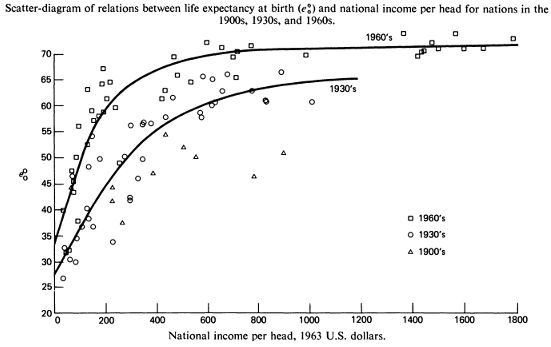
\includegraphics[ height=9cm, width=13cm]{The-original-Preston-Curve-1975.jpg}
\caption{The original Preston curve from \cite{Preston1975}}
\label{Preston}
\end{figure}











\cite{Kalwij2014}

\cite{Oeppen2019} Very Good!!

\cite{Preston1975} is a seminal work according to \cite{Oeppen2019}

inequality \cite{Hu2015}

\cite{Chetty2016} in the US

income inequality does not affect health of a a country \cite{JasonBeckfield2004}

\cite{Tarkiainen2012} (To be downloaded)

\subsubsection{Education atainment}


\cite{Kaplan2015} investigated the relationship between educational atainment and life expectancy in eight states in the United States. They found that even when controlling for variables like income, race, sex and common medical issues like cardiovascular disease, the relationship between educational antainment and life expectance remains statistically significant.

\cite{Luy2019} studied 3 developed nations, namely the United States, Italy and Denmark. They have also found a strong correlation between education levels and longevity.



But what is the nature of this correlation? According to \cite{Deary2004} Intelligence Quotient or IQ could explain the association. While \cite{Hayward2015} does not believe in a ``causal relationship'' but rather that it depends on factors like ``time, place, and the social environment''.

In an attempt to find a causal relationship between education and life expectancy, \cite{VanKippersluis2009} investigated the result of the Netherlands increasing the mandatory number of years a child had to attend school to 7 years. It was 6 years previously. \cite{VanKippersluis2009} found a decrease in mortality of 3\% for 81 year old males who had the additional year of schooling. 

This relationship appears strongest in more developed countries where the life expectancy is already above 60 years \citep{Bulled2010}. In these countries, any educational investment leads to greater compensation for the learner than they would get in a less developed country \cite{Bulled2010,Handwerker1986}. In addition, \cite{Kabir2008} also studied this relationship, among others, with regards to developing countries and did not find a correlation.

The question remains, which educational indicators should be used when investicating the relationship between education and life expectancy?

Various educational indicators have been used in the literature for comparing to life expectancy. One approach is to use the International Classification of Education (ISCED) system \citep{UNESCO2012}. The ISCED 2011 standard consists of 9 levels ranging from ISCED level 0 (Early childhood education) to ISCED level 8 (Doctoral or equivalent level).

\cite{Luy2019} used the United Nations ISCED-97 (consisting of 7 levels) scale to break education attainment down into 3 levels namely Low (None to Lower Secondary), Medium (Upper secondary) and High (Tertiary education). In \cite{VanKippersluis2009} the Dutch SOI system (Standaard Onderwijs Indeling). Which according to \cite{VanKippersluis2009} is similar to the ISCED system. While in \cite{Deboosere2009} educational attainment was broken into 5 levels also ranging from no education to Tertiarty education. 

\cite{Kaplan2015} broke educational attainment into 4 levels ranging from less than high school to college graduate.

In the study \cite{Bulled2010}, the relationship between educational invesments and fertility against life expectancy, over 193 countries, was investigated. They used adult literacy and the enrolment ratios for primary,secondary and tertiary schooling.


For more see \cite{Montez2015} Much information!!!!









helping individuals to mobilise health resources \cite{Elo1996} from \cite{Deboosere2009}





Study in Belgium \cite{Deboosere2009}


Inverse relationship  \cite{Hoque2019}

netherlands \cite{VanKippersluis2009}

\cite{VanBaal2016a}

\subsubsection{Per capita spending on health}

Healthcare spending and life expectancy in the Unites States, between 1960 and 2000, was compared in  \cite{Cutler2006}. They found that the increased spending on health per capita, controlling for inflation, is positively correlated to US life expectancy for the time period in question. 

Most Eastern European countries, who have joined the European Union, have seen an increase in healthcare spending. This has generally been accompanied by an increase in life expectancy \citep{Jakovljevic2016}. This has to be seen in the light of the so called ``Russian Mortality Crisis'' where former Soviet Union countries faced a sudden drop in life expectancy after the fall of the Berlin wall \citep{Brainerd2005}. \cite{Jakovljevic2016} found that the best metric to use when comparing health spending of coutries to be their total per capita health spending in US dollars.

The same relationship was found in Canada. When spending on healthcare is decreased, life expectancy follows \citep{cre}.

It is well known that life expectancy in Sub-Saharan Africa is low. Here spending on health care can also be correlated to increases in life expectancy. Even though poor governance can undo some of the effects of increased spending \citep{Makuta2015}.

A countries per capita healthcare is not neccesarily in proportion to its per capita income. In 2005 the United States spent 50\% more on healthcare per capita than its income per capita would suggest \citep{Anderson2008}.






%Husain, AR (2002), �Life Expectancy in Developing Countries: A Cross-Section Analysis�, The Bangladesh Development Studies, 28(1&2)








\cite{Shaw2005} showed that pharmaceutical expenditures shows a positive correlation with life expectancy in OECD countries.

medical spending \cite{Cutler2006}

?Grossman?
2017 determinants of health: an economic perspective  ????
1972 The Demand for Health: A Theoretical and Empirical Investigation,

\cite{Grossman2000}

\subsubsection{Unemployment}

According to \cite{Bonamore2015}, the literature has 2 main views on the relationship between unemployment and life expectancy. The first view states that during an economic downturn, people suffer from more stress and depression. This leads to more unhealthy lifestyle choices like smoking and alcohol. Which in turn lower life expectancy. \cite{Bonamore2015} cites the works of \cite{Lundin2014,Montgomery2013,GARCY20121911,BROWNING2012599,valos2012,backhans2011unemployment,DEB2011317} and \cite{Strully2009}, who take this view. The second view focusses on times when there is economic growth i.e. less unemployment. This period of economic growth also cal lead to stress eg. burning out and having less time for activities that benifit ones health. Like going to the gym. This view is held by \cite{TapiaGranados2011,RUHM2005341,TapiaGranados2005,NEUMAYER20041037} and \cite{Ruhm2000}. Then there are also studies express the view that no connection can be established \citep{Bonamore2015}. The view of  \cite{Bonamore2015} is that the relationship is non-linear.


unemployment \cite{Bonamore2015} \cite{Roelfs2011} \cite{Roelfs2015} 

\subsection{Cross country studies}

\cite{Bulled2010} Pearsons r and multivariate regression.\cite{Bulled2010} aims to show correlation not prediction.

\cite{Shaw2005} assumes a linear model and uses regression.

\cite{Kabir2008} investigated how well the life expectancy of 93 developing countries were predicted by indicators like income,education and fertility (among others). It classied a countries life expectancy into 3 categories. Then used a probit model where the input variables have a linear relationship. Multiple Ordinary Least Squares Regression was then applied to study inicators' influences.

The study \cite{Hu2015}, also used a linear regression model of GDP per capita, Gini indeces, ect with respect to life expectancy. The intention of the study was to link income inequality to mortality rates and life expectancy.

\subsection{Multi variate studies}

\section{Methodology/Procedure}


This study will attempt to create a model that can predict life expectancy for a country based on various socio-economic conditions in the country. Then evaluate how well various machine learning techniques model the relationships.

The philosophical standpoint of this study is Positivism. By using the scientific method, this study will comprise of an experiment to inductively determine whether machine learning techniques can provide more accurate life expectancy models than those created using regression. This cross-sectional study will use life expectancy indicators shown, from the literature, to have some correlation to life expectancy.



There are many studies that attempt to extrapolate future life expectancy for countries based on current data. This includes studies for high income countries \citep{Kontis2017} and low income countries ????{cite}.

segment data into groups where each group has the same amount of data points???

Unlike \cite{Shaw2005}, this study will not take into account the age distribution of each country.

As for HDI from \cite{Bulled2010}
Adult literacy rate

primary secondary and tertiary enrolment ratios

GDP per Capita (Purchasing power parity )


``National datasets must be regarded with some level of caution as data gaps and issues of inconsistency and incoherence remain owing to differences in the effectiveness of infrastructure, political agendas, and additional factors, such as internal conflicts'' \cite{Bulled2010}  


The impact of finishing secondary school is different before vs after the second world war \cite{Deboosere2009}

\subsection{Choice of dataset}

\subsubsection{Life Expectancy}
For life expectancy data, this study will use the indicator ``Life expectancy at birth, total(years) \{SP.DYN.LE00.IN\}'' from the World Bank's Development Indicators Database \citep{WDI}. This is a weighted average combining both male and female life expectancy and is calculated in a period life table (see Section \ref{LifeExpectancy}). Only the data that is available for the last 30 years (1988-2017) will be used. This is in keeping with other studies where the amount of years that their studies look back on is limited to relatively recently \citep{Luy2019, Hu2015,Tarkiainen2012,Kabir2008, Shaw2005}. 

\subsubsection{Income}

This study will use GDP per capita as was used in \cite{Oeppen2019,Shkol2019,Mackenbach2013} and \cite{DeVogli2005}. The source will be GDP per capita, PPP (constant 2011 international \$)\{NY.GDP.PCAP.PP.KD\} from the World Bank \citep{WorldBank_gdp}.

\subsubsection{Educational Atainment}

Just as in \cite{Bulled2010}, this study will use adult literacy, and primary, secondary and tertiary enrolment ratios. For adult literacy indicator SE.ADT.LITR.ZS will be used from the world bank website \citep{adultLiteracy}. The world bank credits UNESCO for the data. The indicator describes the percentage of adults, from the eage of 15, who can read and write to a certain level of proficiency.  





\subsection{Choise of algorithms}

\subsubsection{Algorithms Chosen}
\paragraph{Regression} \label{regression}
Linear Regression is a popular technique, used to find relationships in data. As the name suggests Linear Regression assumes a linear relationship between the input variables and the result \citep{Murphy}. This might not be the case for the target function. The target function could be any potential function. In the case of life expectancy modelling, we know that according to the Preston curve (Section \ref{income}) the relationship between income and life expectancy is not linear. Thus using Linear Regression should return a sub-optimal result. The same logic applies to Logistic Regression. It assumes a linear relationhip between inputs. The difference is that this linear sum is passed through the sigmoid function \citep{Murphy}. This alsom makes it inappropriate for non-linear target functions. In this study Linear and Logistic Regression will be used as a baseline for comparison on the dataset.

\paragraph{Ridge Regression}

\paragraph{k-Nearest Neighbour}

The k-Nearest Neighbour algorithm (kNN) is an instance based form of machine learning. It uses the classification of those datapoints closest to the datapoint to be classied to determine its classification. The kN-algorithm allows for non-linear problems spaces to be classified, because it does not make an assumption on the nature of the problem space. Additionally, how the algorithm determined its output value is transparent and can be used to study how various components affects the end result. In this study the standard kNN-algoritm will be altered to accomodate a real valued output and not just a class classification. This will be accomplised by taking the mean life expectancy for all the datapoints determined to be closest to the target point. Care will have to be taken to reduce the number of features the data, because this algorithm is sensitive to the so-called ``curse of dimentionality'' \citep{Mitchell}.

using PCA to reduce dimentions

compare different distance metrics 

can be used to determine missing data
\paragraph{Support Vector Machines}

The classic Support Vector Machine (SVM) is used in classification tasks. It involves determining the decision surface with regards to the datapoints closest to the surface. This study will use a modified SVM algorithm that makes it usefull for regression tasks. The SVN regression is described in \cite{smola2004}. The final model can be descriped as:

\begin{equation}
 f(x) = \sum_{i=1}^l (\alpha_i-\alpha_i^*)k(x_i,x)+b
\end{equation}

where $\alpha_i$ and $\alpha_i^*$ are Lagrange multipliers, $b$ is the bias and the term $k(x_i,x)$ is the kernel. The kernel is a function to determine the similarity between 2 input vectors. Various kernels will be investigated, including the Radial-basis function

\begin{equation}
 k(x_i,x) = exp(-\frac{\mid\mid x-x_i \mid\mid^2}{2\sigma^2})
\end{equation}

and the polynomial kernel

\begin{equation}
 k(x_i,x) = (x_i.x +1)^p
\end{equation}


\subsubsection{Ignored Algorithms}
\paragraph{Neural Networks}
Even though Neural networks are capable of representing non-linear hypothesis spaces \citep{Mitchell}, theyare not appropriate for this study for a couple of reasons. Firsly, the datasets that are available are not large enough. Neural networks typically require thousands if not tens of thousands of datapoints. Secondly the amount of processing power and processing time required, will not be available to this study. Thirdly, the results of nural networks are hard to interperet. How the Neural Network came to its conclusion is not clear to the researcher. Which makes it unsuitable as a tool to study the relationship between life expectancy and its various indicators.

\paragraph{Decision Trees}

Traceability and understandability are some of the hallmarks of Decision Trees. These algorithms are well suited problem spaces where the target function and the input attributes are discrete values. It is possible to approximate continuous input attributes by making a branch in the tree when a value is smaller or greter than some value or is between some value. For functions where input attributes span over large ranges, this leads to very large and sub-optimum trees \citep{Mitchell}. The problem of determining life expectancy from socio-economic indices has a continuous target function output and continuous input attributes. Therefor, Decision Trees will be excluded from this study.

\paragraph{Clustering}

Clustering techniques are a form of unsupervised learning where the algorithm tries to group the data in a number of groups. Inessence, classifying the data into categories. This study will not attempt to classify the data, but rather find appropirate machine learning algorithms that could replce linear and logistic regression. While at the same time being able to predict the output of an input vector without needing to classify it first.

\paragraph{Bayes}








\subsection{Cross-validation}

By using stratified \textit{k}-fold cross validation, this study will aim to reduce the impact of the relative small dataset that will be analysed. This form of cross validation will ensure that when the validation set is chosen, no important datapoints are ignored for training. The data will be broken down randomly into \textit{k} subsets of equal size. Each data subset will also contain equal amounts of datapoints with low and high life expectancies, so that no dataset is completely towards one end of the data range. One data subset is chosen to be the validation subset and the remaining $\textit{k} - 1$ subsets are combined into the training set. The model is then trained on the training dataset andt its performance is measured against the validation subset. This is done \textit{k} times in order for each subset to be the validation subset. For each of the training runs the mean of the error will be calculated \citep{Mitchell,Murphy}. The value of \textit{k} will be dependant on the final dataset. 

















%\section{Analysis}


%\cite{Murphy} p23 how to compare techniques
%\section{Conclusion}

%\section{Recommendations}


\appendix
\appendixpage

\begin{longtable}{|c|c|c|c|c|c|c|}
\caption{Life table for the total population: United States, 2003 \citep{Arias2007}}
    \label{LifeTable}\\
 \hline 
      &               &              &               &               & Total        &              \\
       & Probability   &              & Number        & Person-years  & number of    &              \\
       & of dying      & Number       & dying         & lived         & person-years & Expectation  \\
       & between       & surviving to & between       & between       & lived above  & of life      \\
       & ages x to x+1 & age x        & ages x to x+1 & ages x to x+1 & age x        & at age x     \\
\hline  
Age    & q(x)          & l(x)         & d(x)          & L(x)          & T(x)         & e(x)         \\
\hline 
0-1    & 0.006865      & 100,000      & 687           & 99,394        & 7,743,016    & 77.4         \\
1-2    & 0.000469      & 99,313       & 47            & 99,290        & 7,643,622    & 77.0         \\
2-3    & 0.000337      & 99,267       & 33            & 99,250        & 7,544,332    & 76.0         \\
3-4    & 0.000254      & 99,233       & 25            & 99,221        & 7,445,082    & 75.0         \\
4-5    & 0.000194      & 99,208       & 19            & 99,199        & 7,345,861    & 74.0         \\
5-6    & 0.000177      & 99,189       & 18            & 99,180        & 7,246,663    & 73.1         \\
6-7    & 0.000160      & 99,171       & 16            & 99,163        & 7,147,482    & 72.1         \\
7-8    & 0.000147      & 99,156       & 15            & 99,148        & 7,048,319    & 71.1         \\
8-9    & 0.000132      & 99,141       & 13            & 99,134        & 6,949,171    & 70.1         \\
9-10   & 0.000117      & 99,128       & 12            & 99,122        & 6,850,036    & 69.1         \\
10-11  & 0.000109      & 99,116       & 11            & 99,111        & 6,750,914    & 68.1         \\
11-12  & 0.000118      & 99,105       & 12            & 99,100        & 6,651,803    & 67.1         \\
12-13  & 0.000157      & 99,094       & 16            & 99,086        & 6,552,704    & 66.1         \\
13-14  & 0.000233      & 99,078       & 23            & 99,067        & 6,453,618    & 65.1         \\
14-15  & 0.000339      & 99,055       & 34            & 99,038        & 6,354,551    & 64.2         \\
15-16  & 0.000460      & 99,022       & 46            & 98,999        & 6,255,513    & 63.2         \\
16-17  & 0.000577      & 98,976       & 57            & 98,947        & 6,156,514    & 62.2         \\
17-18  & 0.000684      & 98,919       & 68            & 98,885        & 6,057,566    & 61.2         \\
18-19  & 0.000769      & 98,851       & 76            & 98,813        & 5,958,681    & 60.3         \\
19-20  & 0.000832      & 98,775       & 82            & 98,734        & 5,859,868    & 59.3         \\
20-21  & 0.000894      & 98,693       & 88            & 98,649        & 5,761,134    & 58.4         \\
21-22  & 0.000954      & 98,605       & 94            & 98,558        & 5,662,485    & 57.4         \\
22-23  & 0.000990      & 98,511       & 98            & 98,462        & 5,563,928    & 56.5         \\
23-24  & 0.000997      & 98,413       & 98            & 98,364        & 5,465,466    & 55.5         \\
24-25  & 0.000982      & 98,315       & 97            & 98,267        & 5,367,101    & 54.6         \\
25-26  & 0.000960      & 98,219       & 94            & 98,171        & 5,268,835    & 53.6         \\
26-27  & 0.000942      & 98,124       & 92            & 98,078        & 5,170,663    & 52.7         \\
27-28  & 0.000936      & 98,032       & 92            & 97,986        & 5,072,585    & 51.7         \\
28-29  & 0.000947      & 97,940       & 93            & 97,894        & 4,974,599    & 50.8         \\
29-30  & 0.000974      & 97,847       & 95            & 97,800        & 4,876,705    & 49.8         \\
30-31  & 0.001008      & 97,752       & 98            & 97,703        & 4,778,906    & 48.9         \\
31-32  & 0.001046      & 97,654       & 102           & 97,603        & 4,681,203    & 47.9         \\
32-33  & 0.001097      & 97,551       & 107           & 97,498        & 4,583,600    & 47.0         \\
33-34  & 0.001162      & 97,444       & 113           & 97,388        & 4,486,102    & 46.0         \\
34-35  & 0.001244      & 97,331       & 121           & 97,271        & 4,388,715    & 45.1         \\
35-36  & 0.001336      & 97,210       & 130           & 97,145        & 4,291,444    & 44.1         \\
36-37  & 0.001441      & 97,080       & 140           & 97,010        & 4,194,299    & 43.2         \\
37-38  & 0.001567      & 96,940       & 152           & 96,864        & 4,097,289    & 42.3         \\
38-39  & 0.001714      & 96,788       & 166           & 96,705        & 4,000,424    & 41.3         \\
39-40  & 0.001874      & 96,623       & 181           & 96,532        & 3,903,719    & 40.4         \\
40-41  & 0.002038      & 96,442       & 197           & 96,343        & 3,807,187    & 39.5         \\
41-42  & 0.002207      & 96,245       & 212           & 96,139        & 3,710,844    & 38.6         \\
42-43  & 0.002389      & 96,033       & 229           & 95,918        & 3,614,705    & 37.6         \\
43-44  & 0.002593      & 95,803       & 248           & 95,679        & 3,518,787    & 36.7         \\
44-45  & 0.002819      & 95,555       & 269           & 95,420        & 3,423,108    & 35.8         \\
45-46  & 0.003064      & 95,285       & 292           & 95,139        & 3,327,688    & 34.9         \\
46-47  & 0.003322      & 94,993       & 316           & 94,836        & 3,232,548    & 34.0         \\
47-48  & 0.003589      & 94,678       & 340           & 94,508        & 3,137,713    & 33.1         \\
48-49  & 0.003863      & 94,338       & 364           & 94,156        & 3,043,205    & 32.3         \\
49-50  & 0.004148      & 93,974       & 390           & 93,779        & 2,949,049    & 31.4         \\
50-51  & 0.004458      & 93,584       & 417           & 93,375        & 2,855,270    & 30.5         \\
51-52  & 0.004800      & 93,167       & 447           & 92,943        & 2,761,895    & 29.6         \\
52-53  & 0.005165      & 92,719       & 479           & 92,480        & 2,668,952    & 28.8         \\
53-54  & 0.005554      & 92,241       & 512           & 91,984        & 2,576,472    & 27.9         \\
54-55  & 0.005971      & 91,728       & 548           & 91,454        & 2,484,487    & 27.1         \\
55-56  & 0.006423      & 91,181       & 586           & 90,888        & 2,393,033    & 26.2         \\
56-57  & 0.006925      & 90,595       & 627           & 90,281        & 2,302,145    & 25.4         \\
57-58  & 0.007496      & 89,968       & 674           & 89,630        & 2,211,864    & 24.6         \\
58-59  & 0.008160      & 89,293       & 729           & 88,929        & 2,122,234    & 23.8         \\
59-60  & 0.008927      & 88,565       & 791           & 88,169        & 2,033,305    & 23.0         \\
60-61  & 0.009827      & 87,774       & 863           & 87,343        & 1,945,136    & 22.2         \\
61-62  & 0.010831      & 86,911       & 941           & 86,441        & 1,857,793    & 21.4         \\
62-63  & 0.011872      & 85,970       & 1021          & 85,460        & 1,771,352    & 20.6         \\
63-64  & 0.012891      & 84,949       & 1095          & 84,402        & 1,685,892    & 19.8         \\
64-65  & 0.013908      & 83,854       & 1166          & 83,271        & 1,601,490    & 19.1         \\
65-66  & 0.015003      & 82,688       & 1241          & 82,068        & 1,518,219    & 18.4         \\
66-67  & 0.016267      & 81,448       & 1325          & 80,785        & 1,436,151    & 17.6         \\
67-68  & 0.017699      & 80,123       & 1418          & 79,414        & 1,355,366    & 16.9         \\
68-69  & 0.019320      & 78,705       & 1521          & 77,944        & 1,275,953    & 16.2         \\
69-70  & 0.021108      & 77,184       & 1629          & 76,369        & 1,198,008    & 15.5         \\
70-71  & 0.022950      & 75,555       & 1734          & 74,688        & 1,121,639    & 14.8         \\
71-72  & 0.024904      & 73,821       & 1838          & 72,902        & 1,046,951    & 14.2         \\
72-73  & 0.027151      & 71,982       & 1954          & 71,005        & 974,050      & 13.5         \\
73-74  & 0.029784      & 70,028       & 2086          & 68,985        & 903,044      & 12.9         \\
74-75  & 0.032753      & 67,942       & 2225          & 66,830        & 834,059      & 12.3         \\
75-76  & 0.035831      & 65,717       & 2355          & 64,540        & 767,230      & 11.7         \\
76-77  & 0.038987      & 63,362       & 2470          & 62,127        & 702,690      & 11.1         \\
77-78  & 0.042503      & 60,892       & 2588          & 59,598        & 640,563      & 10.5         \\
78-79  & 0.046557      & 58,304       & 2714          & 56,947        & 580,965      & 10.0         \\
79-80  & 0.051200      & 55,589       & 2846          & 54,166        & 524,019      & 9.4          \\
80-81  & 0.056335      & 52,743       & 2971          & 51,258        & 469,853      & 8.9          \\
81-82  & 0.061837      & 49,772       & 3078          & 48,233        & 418,595      & 8.4          \\
82-83  & 0.067856      & 46,694       & 3168          & 45,110        & 370,362      & 7.9          \\
83-84  & 0.074504      & 43,526       & 3243          & 41,904        & 325,252      & 7.5          \\
84-85  & 0.081975      & 40,283       & 3302          & 38,632        & 283,348      & 7.0          \\
85-86  & 0.089682      & 36,981       & 3317          & 35,322        & 244,716      & 6.6          \\
86-87  & 0.098031      & 33,664       & 3300          & 32,014        & 209,394      & 6.2          \\
87-88  & 0.107059      & 30,364       & 3251          & 28,739        & 177,380      & 5.8          \\
88-89  & 0.116804      & 27,113       & 3167          & 25,530        & 148,641      & 5.5          \\
89-90  & 0.127300      & 23,946       & 3048          & 22,422        & 123,111      & 5.1          \\
90-91  & 0.138581      & 20,898       & 2896          & 19,450        & 100,689      & 4.8          \\
91-92  & 0.150676      & 18,002       & 2712          & 16,646        & 81,239       & 4.5          \\
92-93  & 0.163611      & 15,289       & 2502          & 14,039        & 64,594       & 4.2          \\
93-94  & 0.177408      & 12,788       & 2269          & 11,654        & 50,555       & 4.0          \\
94-95  & 0.192080      & 10,519       & 2021          & 9,509         & 38,901       & 3.7          \\
95-96  & 0.207636      & 8,499        & 1765          & 7,616         & 29,392       & 3.5          \\
96-97  & 0.224075      & 6,734        & 1509          & 5,980         & 21,776       & 3.2          \\
97-98  & 0.241387      & 5,225        & 1261          & 4,594         & 15,796       & 3.0          \\
98-99  & 0.259552      & 3,964        & 1029          & 3,449         & 11,202       & 2.8          \\
99-100 & 0.278539      & 2,935        & 818           & 2,526         & 7,752        & 2.6          \\
100+   & 1.00000       & 2,118        & 2118          & 5,226         & 5,226        & 2.5          \\
\hline
\end{longtable}


\addappheadtotoc
\addcontentsline{toc}{section}{References}
\bibliography{mybib}



\end{document}
